% !TEX encoding = UTF-8 Unicode

\documentclass[a4paper]{article}

\usepackage{color}
\usepackage{url}
\usepackage[T2A]{fontenc} % enable Cyrillic fonts
\usepackage[utf8]{inputenc} % make weird characters work
\usepackage{graphicx}

\usepackage[english,serbian]{babel}
%\usepackage[english,serbianc]{babel} %ukljuciti babel sa ovim opcijama, umesto gornjim, ukoliko se koristi cirilica

\usepackage[unicode]{hyperref}
\hypersetup{colorlinks,citecolor=green,filecolor=green,linkcolor=blue,urlcolor=blue}

%\newtheorem{primer}{Пример}[section] %ćirilični primer
\newtheorem{primer}{Primer}[section]

\begin{document}


\title{Tehnološka singularnost\\ \small{Seminarski rad u okviru kursa\\Tehničko i naučno pisanje\\ Matematički fakultet}}

\author{Nikola Ahac\\ Dimitrije Petronijević\\ Mladen Radojević\\ Lazar Stošić}
\date{~Novembar 2022.}
\maketitle



\tableofcontents

\newpage

\section{Uvod}
\label{sec:uvod}
Tehnološku singularnost naučnici koriste kako bi označili hipotetički trenutak u budućnosti nakon koga će tehnološki napredak ubrzati I postati toliko komplikovan da će postati nedostupan našem razumevanju. Ovaj termin je prvobitno predložio američki matematičar I pisac naučne fantastike Vernor Vinge 1993. godine. Njegova ideja glasi ovako: Kada čovek stvori mašinu koja je pametnija od čoveka, budućnost će postati nepredvidiva, jer je nemoguće predviddeti ponašanje inteligencije koja je superiornija od čoveka. Vinge predviđa da do ovoga može doći negde u prvoj trećini 21. veka, negde između 2005. i 2003. godine. 

Ovo može dovesti do dva scenarija po našu civilizaciju. Prvi jeste scenario sličan onom u filmu “Matrix” u kome bi mašine pokušale da nas unište, a ddrugi jeste onaj optimističniji u kome bi ljudi i mašine živeli u miru. Mi ne možemo znati do čega će nas dovesti ovaj fenomen niti kada će taj trenutak doći.

\section{Eksplozija inteligencije}
I ako se tehnološki napredak ubrzava uvećini oblasti danas, on je dosta ograničen inteligencijom ljudskog mozga, koja se prema Pol R. Erlihu, nije značajno unapredila milenijumima.\cite{ref 1}Međutim napretkom informacioniih tehnologija i samih računara, u nekoj skorijoj budućnsti može se napraviti mašina koja je znatno inteligentnija od ljudi .\cite{ref 2}

Ako bi se i konstruisala nadljudska inteligencija, bilo to poboljšanjem ljudske inteligencije ili stvaranjem nove veštačke inteligencije, to bi moglo dovesti do toga da se stvori mašina koja je u sposobnosti da sama sebe nadogradjuje, i kroz vreme bi taj proces postajao sve brži i brži do trenutka kada više nebi mogao da se isprati.

Pojam „Eksplozije inteligencije“ je 1965. prvi put pomenuo I.J. Good\cite{ref 3}

\begin{itemize}
\item Neka ultrainteligentna mašina bude definisana kao mašina koja može daleko nadmašiti sve intelektualne aktivnosti bilo kog čoveka koliko god da je pametan. Pošto je projektovanje mašina jedna od ovih intelektualnih aktivnosti, ultrainteligentna mašina bi mogla da dizajnira još bolje mašine; tada bi nesumnjivo došlo do „eksplozije inteligencije“ i inteligencija čoveka bi ostala daleko iza. Tako je prva ultrainteligentna mašina poslednji izum koji čovek treba da napravi, pod uslovom da je mašina dovoljno poslušna da nam kaže kako da je držimo pod kontrolom.
\end{itemize} 
\section{Kako i kada će doći do singularnosti}	
\label{sec:kakoikada}
To kako i kada će doći do singularnosti niko ne može sa sigurnošću tvrditi, postoje mnoge pretpostavke i ideje, ali se takva stvar jednostavno ne može predvideti.

U daljem tekstu će biti predstavljeno par takvih ideja.
\subsection{Pojava superingelencije}

Superinteligencija, hiperinteligencija ili nadljudska inteligencija je pojam koji se odnosi na neku vrstu veštačke inteligencije koja daleko nadmašuje inteligenciju ljudskog mozga.  John von Neumann, Vernor Vinge i Rej Kurzwelli smatraju da je današnjem čoveku nemoguće da predvidi kakve će posledice po njega imati nastanak „Supre inteligencije“.\cite{ref 4}\cite{ref 5}
Međutim neki tehnološki prognostičari i istraživači se ne slažu oko toga kada će i da li će ljudska inteligencija biti nadmašena.  Neki tvrde da će napredak u veštačkoj inteligenciji verovatno rezultirati opštim sistemima rasuđivanja koji zaobilaze ljudska kognitivna ograničenja. Drugi veruju da će ljudi evoluirati ili direktno modifikovati svoju biologiju kako bi postigli radikalno veću inteligenciju.\cite{ref 6}\cite{ref 7}
Brojni scenariji studija budućnosti kombinuju ove mogućnosti, sugerišući da će se ljudi verovatno povezati sa računarima ili preneti svoje umove na računare, na način koji omogućava značajno povećanje inteligencije. Knjiga The Age of Em od Robina Hansona opisuje budućnost u kojoj se pojavljuju ljudski mozgovi umesto ili na putu do pojave superinteligencije\cite{ref 8}

\subsection{Singularnost bez veštačke inteligencije}

Neki naučnici koriste „singularnost“ na širi način tako što upućuju na bilo kakve radikalne promene u našem društvu izazvane novim tehnologijama kao što je molekularna nanotehnologija,\cite{ref 9}\cite{ref 10}\cite{ref 11}iako Vinge i drugi naučnici posebno navode da bez superinteligencije, takve promene se ne bi kvalifikovale kao prava singularnost.

\subsection{Brza superinteligencija}
Brza superinteligencija opisuje veštačku inteligenciju koja može da funkcioniše kao ljudski um, samo dosta brže\cite{ref 12}Na primer, sa milion puta povećanom brzinom obrade informacija u odnosu na ljude, subjektivna godina bi prošla za 30 fizičkih sekundi. Takva razlika u brzini obrade informacija mogla bi da pokrene singularnost.

\section{Verovatnoća da će doći so singularnosti}	
\label{sec:verovatnoća}
Nekoliko istaknutih tehnologa i akademika je diskutovalo o mogućnosti da se singularnost ostvari. 

Većina njih predlaže da do singularnosti može doći na jedan od dva načina: veštačkom inteligencijom i amplifikacijom ljudskog mozga, za koju su neke od predloženih metoda bioinženjering, genetski inženjering, AI asistenti, različite vrste droga, direktna veza mozga i računara, kao i "upload-ovanje" mozga na računar. Računajući da se konstantno radi na istraživanju ovakvih grana, mogućnost da dođemo do singularnosti se samo povećava. \cite{mog-1}

Tri glavna faktora koji utiču na ostvarivanje singularnosti su: \cite{mog-2}
\begin{itemize}
\item Prvi, ubrzavajući, faktor su poboljšivači inteligencije, koji se konstantno nadograđuju na svoje predhodnike 
\item Drugi, nasuprot prvom, je usporavajući faktor i on je otežavanje napretka time što je tehnologija sve naprednija. U jednom momentu će se možda doći da će komplikacije u razvoju prevazići potencijalni napredak inteligencije
\item Treći, isto usporavajući, je eventualna fizička granica, gde zakoni fizike neće dozvoljavati dalji napredak  
\end{itemize} 
U online anketi iz 2017. godine, na pitanje koliko je verovatno da dođe do eksplozije inteligencije, 12\% ispitanika je reklo da će "vrlo verovatno" doći do iste, 17\% ispitanika je reklo "verovatno", 21\% ispitanika je reklo "možda", 24\% ispitanika je reklo "malo verovatno", a 26\% ispitanika je reklo da je to "skoro nemoguće". \cite{mog-3}

\subsection{Razvoj brzine tehnološkog napretka}

Murov zakon (eng.~{\em Moore's law}), je opažanje da se broj tranzistora po jedinici prostora duplira na svake dve godine. 

Analogija Murovom zakonu je da ako bi za prvo dupiranje brzine hardvera računara trebalo 18 meseci, sa sledeće bi trebalo 9, posle čega bi trebalo četiri, pa dva, jedan i tako dalje dok se eventualno ne bi došlo do neke gornje granice za brzinu. \cite{mog-4}

Džef Hokins (eng.~{\em Jeff Hawkins}) je rekao da bi samopoboljšavajući računarski sistem eventualno došao do neke gornje granice računarske snage : "postoji granica koliko brzi i veliki računari mogu da postanu. U svakom slučaju, završićemo na istoj tački, možda samo malo brže. Ne bi došlo do singularnosti". \cite{mog-5}

\begin{figure}[h!]
\begin{center}
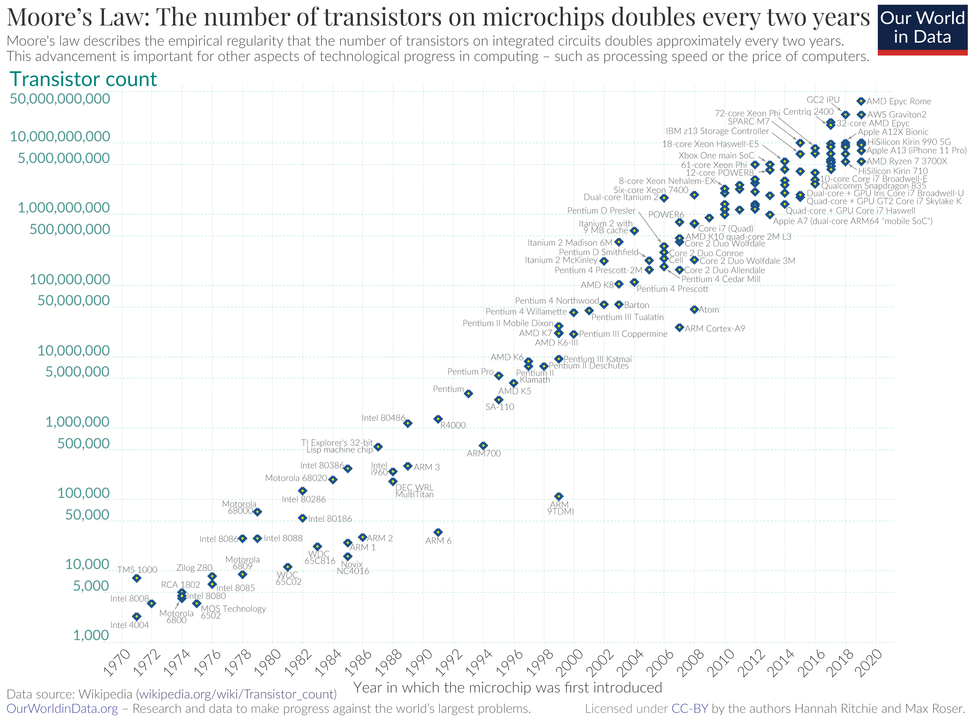
\includegraphics[scale=0.35]{moore.png}
\end{center}
\caption{Murov zakon}
\label{fig:frog}
\end{figure}

Eksponencijalni napredak predložen u Murovom zakonu se koristi kao jedan od glavnih pokazatelja da rezumno očekivati dolazak singularnosti u skorijoj budućnosti.

Rej Kurcvail (eng.~{\em Jeff Hawkins}) predlaže zakon o ubrzanom povratku, generalizujuću Murov zakon na celokupnu tehnologiju i govori o tome da se brzina tehnološkog razvoja eksponencijalno povećava. Taj zakon primenjuje i na tehnologije kao što su materijalna, medicinska i druge. \cite{mog-6}

Kurcvail takođe veruje da će se singularnost desiti do 2045. godine, jer smatra da će tada veštačka inteligencija nadjačati ukupnu sumu moždanog kapaciteta celog čovečanstva. \cite{mog-6}


\subsection{Razvoj algoritama}

Neke tehnologije, kao 'seed AI' \cite{mog-7}, imaju potencijal da se ne samo ubrzaju, već i da poboljšaju svoju efikasnost promenom sopstvenog izvornog koda. 
Ovaj mehanizam se od čistog povećanja brzine izvršavanja razlikuje u dva pogleda.

Prvo, za njega nije potreban spoljni uticaj. Za razliku od hardverskog ubrzavanja, gde je potreban bar neki nivo interakcije od strane čoveka, u ovom mehanizmu AI sam menja sopstveni kod.

Drugo, kao po Vernor Vindžovom (eng.~{\em Vernor Vinge}) viđenju singularnosti, ovaj pristup može biti vrlo nepredvidiv. \cite{mog-8}

\subsection{Kritike}

Neki kritičari, kao Hjubert Drejfus (eng.~{\em Hubert Dreyfus}) tvrde da računari i mašine ne mogu dostići nivo ljudske inteligencije, dok neki kao fizičar Stiven Hoking {\em Stephen Hawking}) tvrde da je definicija inteligencije zanemarljiva ukoliko je krajnji rezultat isti. \cite{mog-9}

Martin Ford u svojoj knjzi "The Lights in the Tunnel: Automation, Accelerating Technology and the Economy of the Future" predlaže "tehnološki paradoks", gde tvrdi da do singularnosti neće doći, zato što bi ona dovela do masovne nezaposlenosti i smanjene trgovinske potražnje, jer bi se pokazala efikasnijom od radnika, što bi za uzvrat dovelo do smanjene inicijative da se ulaže u iste tehnologije. \cite{mog-10}



\section{Slike i tabele}
\label{slike_i_tabele}

Slike i tabele treba da budu u svom okruženju, sa odgovarajućim naslovima, obeležene labelom da koje omogućava referenciranje. 

\begin{primer} Ovako se ubacuje slika. Obratiti pažnju da je dodato i 
\begin{verbatim}
\usepackage{graphicx}
\end{verbatim}

\begin{figure}[h!]
\begin{center}
\includegraphics[scale=0.25]{frog.jpg}
\end{center}
\caption{Frog}
\label{fig:frog}
\end{figure}

Na svaku sliku neophodno je referisati se negde u tekstu. Na primer, na slici \ref{fig:frog} prikazane su pande. 
\end{primer}

\begin{primer} I tabele treba da budu u svom okruženju, i na njih je neophodno referisati se u tekstu. Na primer, u tabeli \ref{tab:tabela1} su prikazana različita poravnanja u tabelama.

\begin{table}[h!]
\begin{center}
\caption{Razlčita poravnanja u okviru iste tabele ne treba koristiti jer su nepregledna.}
\begin{tabular}{|c|l|r|} \hline
centralno poravnanje& levo poravnanje& desno poravnanje\\ \hline
a &b&c\\ \hline
d &e&f\\ \hline
\end{tabular}
\label{tab:tabela1}
\end{center}
\end{table}

\end{primer}





\section{Prvi naslov}
\label{sec:naslov1}


Ovde pišem tekst. 
Ovde pišem tekst. 
Ovde pišem tekst. 
Ovde pišem tekst. 
Ovde pišem tekst. 
Ovde pišem tekst. 
Ovde pišem tekst. 
Ovde pišem tekst. 


\subsection{Prvi podnaslov}
\label{subsec:podnaslov1}

Ovde pišem tekst. 
Ovde pišem tekst. 
Ovde pišem tekst. 
Ovde pišem tekst. 
Ovde pišem tekst. 
Ovde pišem tekst. 
Ovde pišem tekst. 

\subsection{Drugi podnaslov}
\label{subsec:podnaslov2}

Ovde pišem tekst. 
Ovde pišem tekst. 
Ovde pišem tekst. 
Ovde pišem tekst. 
Ovde pišem tekst. 
Ovde pišem tekst. 

\section{Drugi naslov}
\label{sec:naslov2}

Ovde pišem tekst. 
Ovde pišem tekst. 
Ovde pišem tekst. 
Ovde pišem tekst. 

\subsection{... podnaslov}
\label{subsec:podnaslovN}

Ovde pišem tekst. 
Ovde pišem tekst. 
Ovde pišem tekst. 
Ovde pišem tekst. 
Ovde pišem tekst. 
Ovde pišem tekst. 

\section{n-ti naslov}
\label{sec:naslovN}

Ovde pišem tekst. 
Ovde pišem tekst. 
Ovde pišem tekst. 
Ovde pišem tekst. 
Ovde pišem tekst. 

\subsection{... podnaslov}
\label{subsec:podnaslovK}

Ovde pišem tekst. 
Ovde pišem tekst. 
Ovde pišem tekst. 
Ovde pišem tekst. 
Ovde pišem tekst. 

\subsection{... podnaslov}
\label{subsec:podnaslovM}

Ovde pišem tekst. 
Ovde pišem tekst. 
Ovde pišem tekst. 
Ovde pišem tekst. 
Ovde pišem tekst. 

\section{Poslednji naslov}
\label{sec:naslovM}

Ovde pišem tekst. 
Ovde pišem tekst. 
Ovde pišem tekst. 
Ovde pišem tekst. 
Ovde pišem tekst. 
Ovde pišem tekst. 
Ovde pišem tekst. 
Ovde pišem tekst. 
Ovde pišem tekst. 

\section{Zaključak}
\label{sec:zakljucak}

Ovde pišem zaključak. 
Ovde pišem zaključak. 
Ovde pišem zaključak. 
Ovde pišem zaključak. 
Ovde pišem zaključak. 
Ovde pišem zaključak. 
Ovde pišem zaključak. 
Ovde pišem zaključak. 
Ovde pišem zaključak. 
Ovde pišem zaključak. 
Ovde pišem zaključak. 
Ovde pišem zaključak. 


\addcontentsline{toc}{section}{Literatura}
\appendix

\iffalse
\bibliography{seminarski} 
\bibliographystyle{plain}
\fi

\begin{thebibliography}{9}

\bibitem{laski2009software} J. Laski and W. Stanley. \emph{Software Verification and Analysis}. Springer- Verlag, London, 2009.

\bibitem{gcc} Free Software Foundation. GNU gcc, 2013. on-line at: http://gcc. gnu.org/.

\bibitem{mog-1} "What is the Singularity? | Singularity Institute for Artificial Intelligence",  \href{https://web.archive.org/web/20110908014050/http://singinst.org/overview/whatisthesingularity/}{Singinst.org}.

\bibitem{mog-2} Hanson, Robin (1998). \href{https://mason.gmu.edu/~rhanson/vc.html#hanson}{"Some Skepticism"}.

\bibitem{mog-3} Grace, Katja; Salvatier, John; Dafoe, Allan; Zhang, Baobao; Evans, Owain (24 May 2017). "When Will AI Exceed Human Performance? Evidence from AI Experts"

\bibitem{mog-4} Eliezer Yudkowsky, 1996 "Staring into the Singularity"

\bibitem{mog-5} https://spectrum.ieee.org/tech-luminaries-address-singularity

\bibitem{mog-6} Ray Kurzweil, The Singularity Is Near, Penguin Group, 2005

\bibitem{mog-7} Yampolskiy, Roman V. "Analysis of types of self-improving software." Artificial General Intelligence. Springer International Publishing, 2015.

\bibitem{mog-8} Eliezer S. Yudkowsky. "Power of Intelligence"

\bibitem{mog-9} Dreyfus & Dreyfus 2000, p. xiv: 'The truth is that human intelligence can never be replaced with machine intelligence simply because we are not ourselves "thinking machines" in the sense in which that term is commonly understood.' Hawking (1998): 'Some people say that computers can never show true intelligence whatever that may be. But it seems to me that if very complicated chemical molecules can operate in humans to make them intelligent then equally complicated electronic circuits can also make computers act in an intelligent way. And if they are intelligent they can presumably design computers that have even greater complexity and intelligence.'

\bibitem{mog-10}
\href{https://www.nytimes.com/2011/03/05/science/05legal.html}{"Armies of Expensive Lawyers, Replaced by Cheaper Software"}.

\bibitem{haltingproblem} A. M. Turing. \emph{On Computable Numbers, with an application to the Entscheidungsproblem}. Proceedings of the London Mathematical Society, 2(42):230–265, 1936.

\bibitem{ref 1}Ehrlich, Paul. The Dominant Animal: Human Evolution and the Environment Archived 2018-10-08 at the Wayback Machine

\bibitem{ref 2}Superbrains born of silicon will change everything. Archived August 1, 2010, at the Wayback Machine

 \bibitem{ref 3}Good, I. J. "Speculations Concerning the First Ultraintelligent Machine", Advances in Computers, vol. 6, 1965. Archived May 1, 2012, at the Wayback Machine
 
  \bibitem{ref 4} Vinge, Vernor. "The Coming Technological Singularity: How to Survive in the Post-Human Era" Archived 2018-04-10 at the Wayback Machine, in Vision-21: Interdisciplinary Science and Engineering in the Era of Cyberspace, G. A. Landis, ed., NASA Publication CP-10129, pp. 11–22, 1993.
  
   \bibitem{ref 5}Ray Kurzweil, The Singularity Is Near, pp. 135–136. Penguin Group, 2005.
\bibitem{ref 6} Pearce, David (2012), Eden, Amnon H.; Moor, James H.; Søraker, Johnny H.; Steinhart, Eric (eds.), "The Biointelligence Explosion", Singularity Hypotheses, The Frontiers Collection, Berlin, Heidelberg: Springer Berlin Heidelberg, pp. 199–238, doi:10.1007/978-3-642-32560-1_11, ISBN 978-3-642-32559-5, retrieved 2022-01-16


\bibitem{ref 7} Gouveia, Steven S., ed. (2020). "ch. 4, "Humans and Intelligent Machines: Co-evolution, Fusion or Replacement?", David Pearce". The Age of Artificial Intelligence: An Exploration. ISBN 978-1-62273-872-4.

\bibitem{ref 8} Gouveia, Steven S., ed. (2020). "ch. 4, "Humans and Intelligent Machines: Co-evolution, Fusion or Replacement?", David Pearce". The Age of Artificial Intelligence: An Exploration. ISBN 978-1-62273-872-4.

\bibitem{ref 9} "h+ Magazine | Covering technological, scientific, and cultural trends that are changing human beings in fundamental ways". Hplusmagazine.com. Archived from the original on 2010-12-23. Retrieved 2011-09-09.

\bibitem{ref 10}  Yudkowsky, Eliezer. The Singularity: Three Major Schools Archived 2018-10-01 at the Wayback Machine.

\bibitem{ref 11} Sandberg, Anders. An overview of models of technological singularity Archived 2011-07-24 at the Wayback Machine

\bibitem{ref 12} Kaj Sotala and Roman Yampolskiy (2017). "Risks of the Journey to the Singularity". The Technological Singularity. The Frontiers Collection. Springer Berlin Heidelberg. pp. 11–23. doi:10.1007/978-3-662-54033-6_2. ISBN 978-3-662-54031-2.
\end{thebibliography}


\appendix
\section{Dodatak}
Ovde pišem dodatne stvari, ukoliko za time ima potrebe.
Ovde pišem dodatne stvari, ukoliko za time ima potrebe.
Ovde pišem dodatne stvari, ukoliko za time ima potrebe.
Ovde pišem dodatne stvari, ukoliko za time ima potrebe.
Ovde pišem dodatne stvari, ukoliko za time ima potrebe.


\end{document}
